\chapter{Gamma-Ray Astronomy}
\label{ch:gamma-ray-astronomy}

Astronomy, being one of the oldest sciences, is a vast field of study dating back to the Babylonians.
From the earliest days of civilization, astronomers have been studying the stars and the planets to
understand the universe. It, therefore, is no surprise that astronomy spawned a great number of discoveries
throughout the centuries. Whereas first observations were made by eye only, we now have access to a multitude
of experiments and telescopes that deepen our understanding of the universe. With the discovery of
\gls{cr} by Victor Hess in the early 20th century, the new field of astroparticle physics was born \cite{longair1981}.

From then on we found many different types of cosmic messengers, the most recent being the discovery of
gravitational waves in 2015 \cite{PhysRevLett.116.061102}.\todo{rewrite this (maybe)}

\begin{figure}
    \centering
    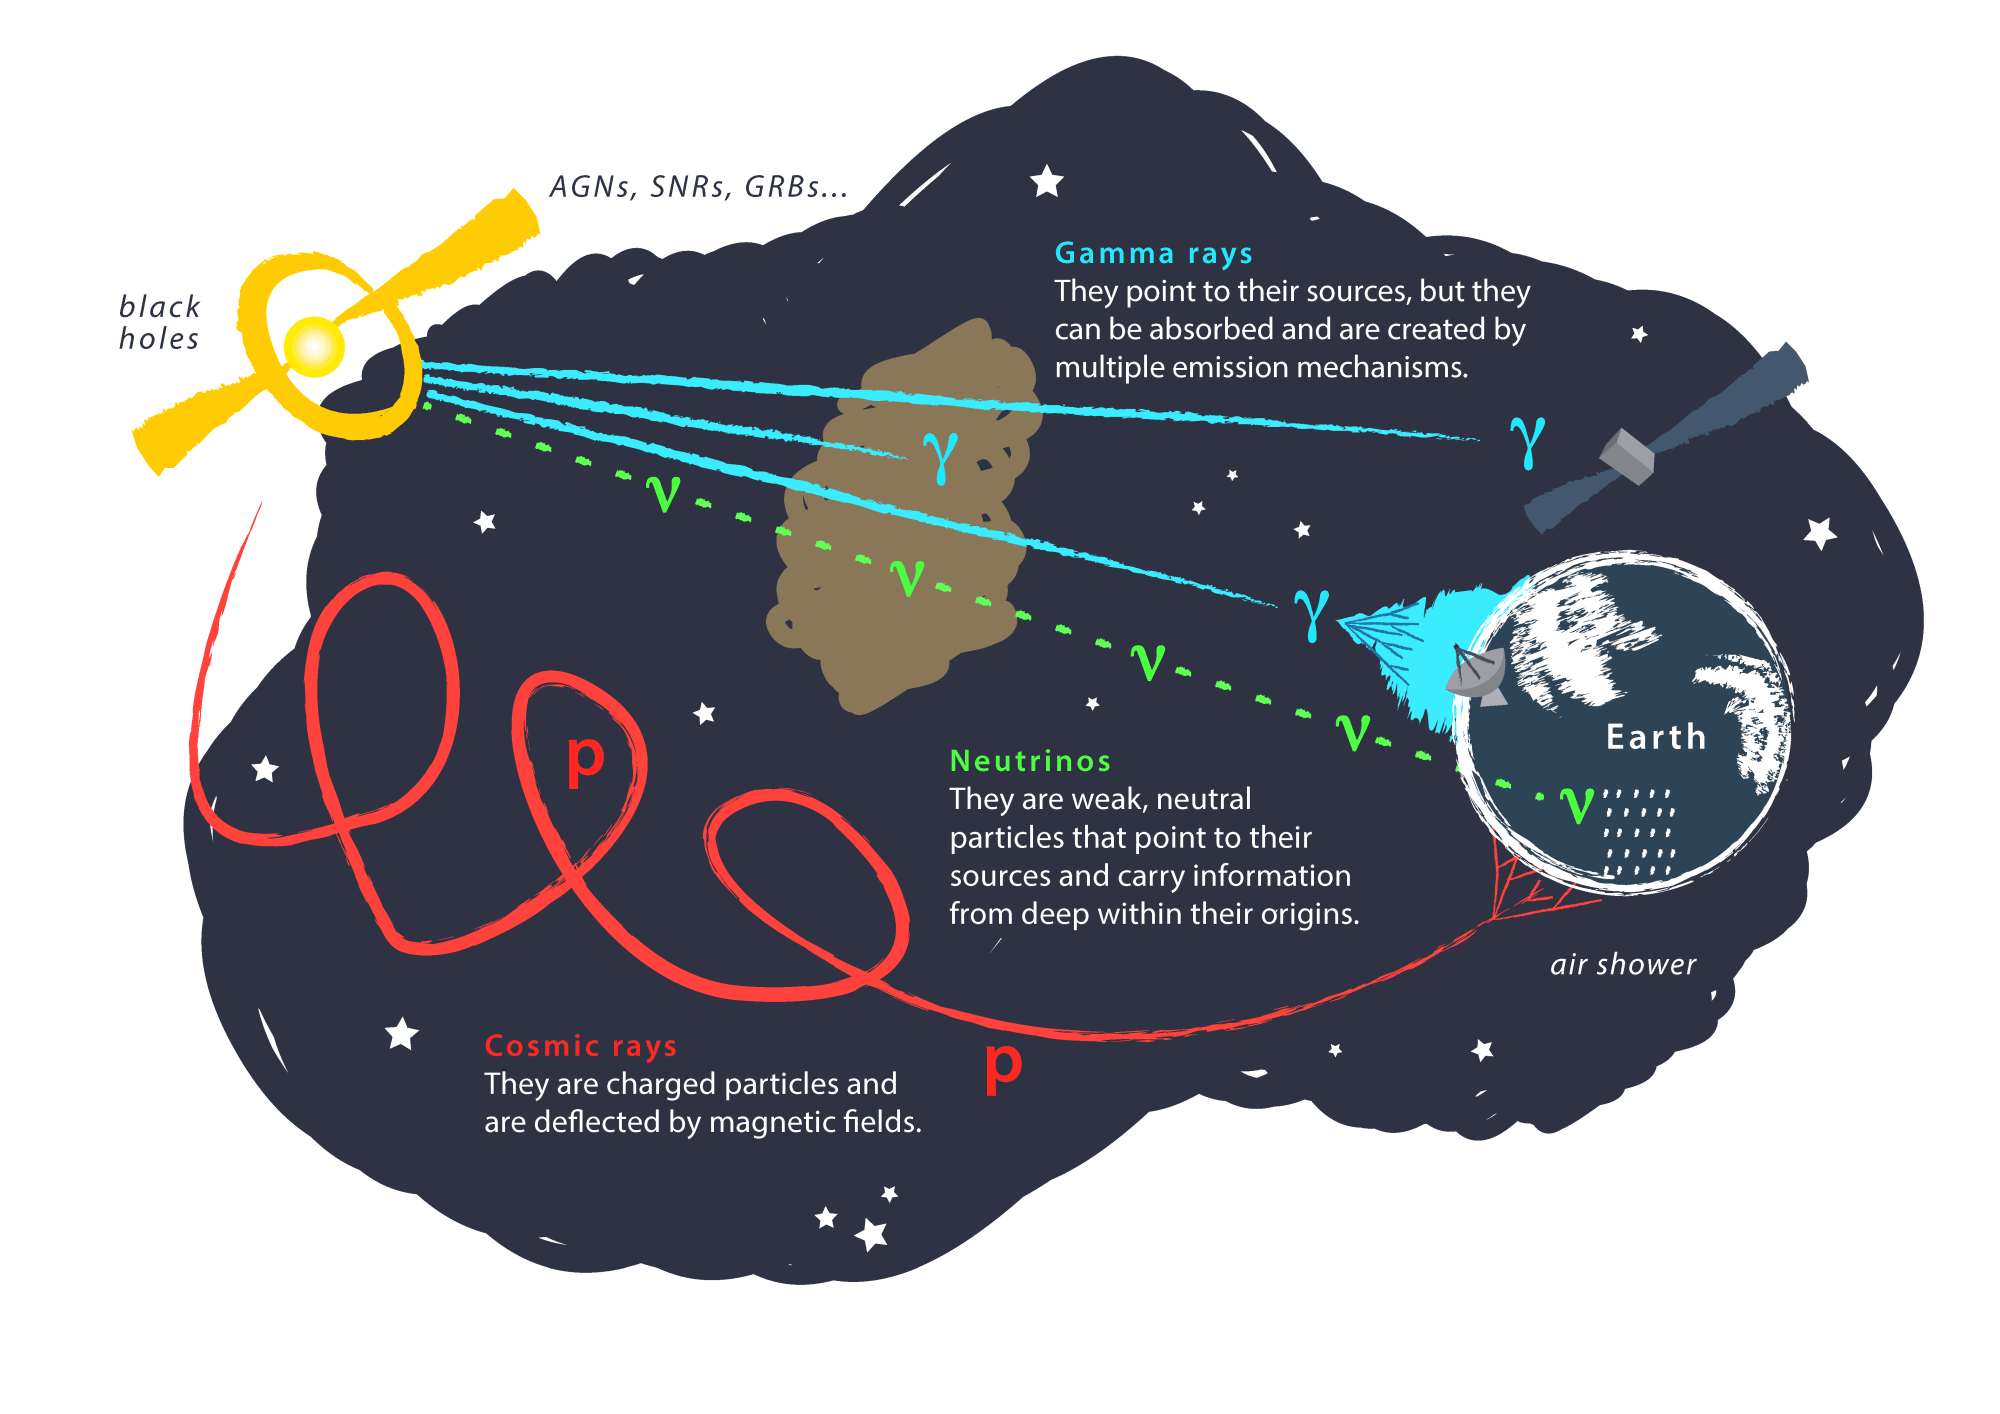
\includegraphics[width=0.8\textwidth]{graphics/figure5.png}
    \caption{Different types of cosmic rays on their way to Earth. Charged particles like protons and electrons
    are deflected by magnetic fields and therefore making it hard to pinpoint the source. Only the
    origin of photons and neutrinos can be reconstructed directly since they are uncharged particles
    and therefore travel in straight lines. However, photons can be absorbed or created in multiple
    mechanisms. Since neutrinos only rarely interact with matter via the weak force, their detection
    is significantly harder than for photons \cite{fig5}.}
    \label{fig:fig5}
\end{figure}

\gls{cr} come in different types, that are either charged or uncharged, as shown in \autoref{fig:fig5}.
Charged particles like electrons, protons or atomic nuclei are difficult to trace back to their origin
as they are deflected by the cosmic electromagnetic fields. Uncharged particles like photons or
neutrinos, however, travel in straight lines, making it easier to reconstruct their origins,
although photons can be absorbed by dust clouds in their way.

Since neutrinos are harder to detect due to their weak interaction with matter, photons are easier to study
with space- and ground-based experiments.

Therefore, in recent years, gamma-ray astronomy has become an important research field in astroparticle physics.
The term gamma-rays is generally denoted as photons with energies above \SI{100}{\kilo\eV}
\cite{funk}. Due to this high-energy nature, gamma rays pose some of the most powerful \gls{cr} in
the universe and since photons at such energies cannot be produced by thermal processes, their origin
can be described by higher order processes involving charged particles. Sources for gamma rays include
\glspl{snr}, Pulsars, Blazars, \glspl{agn} or \glspl{grb}.

\begin{description}
    \item [\glspl{snr}] are the remnants of a supernova explosion.
    \item [Pulsars] are rotating neutron stars that emit gamma rays in the form of pulsations.
    \item [Blazars] are \glspl{agn} that are highly variable and emit gamma rays in the form of
    flares.
    \item [\glspl{agn}] are active galactic nuclei that emit gamma rays in the form of flares.
    \item [\glspl{grb}] are gamma-ray bursts that are the most energetic explosions in the universe.
\end{description}

\begin{figure}
    \centering
    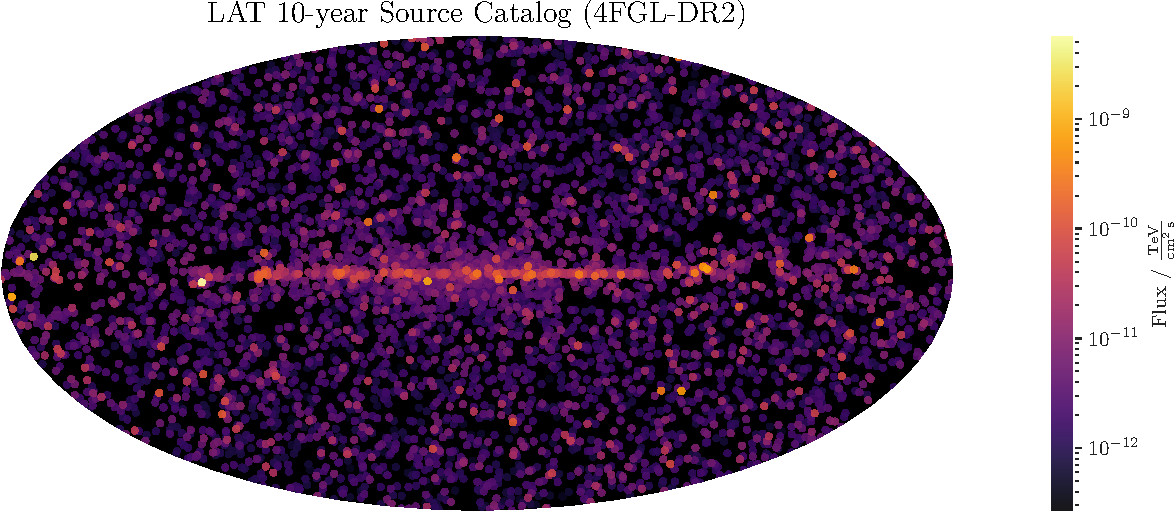
\includegraphics[width=0.8\textwidth]{build/fermi_catalog.pdf}
    \caption{Hammer projection of the Fermi-LAT 4FGL catalog data of gamma-ray sources. The skymap
    shows the flux of gamma-ray sources in \(\si{\tera\eV\per\centi\meter\squared\per\second}\)
    over a span of \(\num{10}\) years \cite{fermi4fgl}.}
    \label{fig:fermilat}
\end{figure}
Gamma rays can be detected by a variety of experiments, either ground- or space-based. Space-based
experiments like the \gls{fermilat} are usually more sensitive to lower energies, whereas ground-based experiments are more
sensitive to higher energies. The \gls{fermilat} is a space-based gamma-ray observatory that was launched
in 2008 and is still in operation today. \autoref{fig:fermilat} shows the gamma-ray sky as observed by the
\gls{fermilat} over a span of \(\num{10}\) years.

For the past two decades, ground-based \gls{iact} experiments like the \gls{magic} telescopes, the
\gls{veritas} and the \gls{hess} have been monitoring these \gls{vhegr} to gain an understanding of
their production. This allowed us to determine different source classes inside and outside our galaxy,
with the most important source class inside our galaxy being \glspl{snr} such as the Crab Nebula.





